% ******************** DEPENDENCIES ********************
\documentclass{article}
\usepackage{graphicx}
\usepackage{hyperref}
\usepackage{amsmath}
\usepackage{amssymb}
\usepackage{float}
\newcommand{\tabitem}{~~\llap{\textbullet}~~}

% ******************** TITLE ********************
\title{BookLocal}

\begin{document}

\maketitle

\begin{flushleft}
\centering PROSPECTUS
\end{flushleft}

% ******************** TOC ********************
\newpage
\tableofcontents

\newpage

% ******************** WHAT ********************
\section{What}
The vision for BookLocal is to connect travelers directly to their hotel of choice by creating the first two way property management system accessible as both a traveler and a hotel administrator. Simply put, BookLocal is designed to remove middlemen from the hotel ecosystem and serve as the single point of contact. Successful implementation allows for three key benefits: simplified user experiences; lower room prices for the traveler; and higher profits for the hotel.  

\begin{flushleft}
At its heart, BookLocal will operate as a series of smart contracts stored on the Ethereum blockchain. To interact with the application, special interfaces for both hotel workers and travelers will be designed to provide full service functionality and replace inefficiencies in the current ecosystem.
\end{flushleft}

\begin{flushleft}
To the traveler, BookLocal will provide the following features:
\begin{itemize}
 \item search;
 \item compare;
 \item book; and
 \item purchase.
\end{itemize}
\end{flushleft}

\begin{flushleft}
To the hotel, BookLocal will provide modules for:
\begin{itemize}
 \item guest management;
 \item housekeeping and maintenance;
 \item revenue management;
 \item payment processing and point of sale;
 \item report generation; and
 \item channel management.
\end{itemize}
\end{flushleft}


\begin{flushleft}
The layout of this paper provides the motivation for BookLocal in section 2, a description of the current ecosystem in section 3, an overview of the features in section 4, and the steps toward full implementation in section 5.
\end{flushleft}


% ******************** WHY ********************
\newpage
\section{Why}
To understand the motivation for BookLocal we identify a few key issues with the current hotel reservation model and propose solutions. 

\subsection{Problems}
The hotel booking industry is fragmented with no fewer than five different groups working for commission between travelers and hotels. Problems include:

\subsubsection*{High commission payments.}
  	\begin{itemize}
	 \item Online travel agents (OTA) receive 15-25\% commission per room.
	 \item Other necessary software packages (i.e. channel manager and property management systems) also require monthly usage fees. 
	 \item These additional payments increase rates for travelers while lowering profit for the hotels.
	\end{itemize}
\subsubsection*{Abuse of power in legal agreements.}
    	\begin{itemize}
	 \item \underline{\textit{Last available room}} clause requires hotels to give the OTA access their last room(s) when near capacity. Because of the high commission rates, this can cause hotels to pass on revenue from more profitable booking options (i.e. last minute walk-ins).
	 \item \underline{\textit{Rate parity}} clause forbids the hotel from renting a room at a lower price through any other source, including their own website, from which they could charge a lower price to the traveler and still receive higher profit. 
	 \item \underline{\textit{Blanket use of trademark rights}} allows an OTA to bid on google ad-words for higher listing than the hotel's brand website.
	\end{itemize}
 \subsubsection*{Fragmented computer systems.}
    	\begin{itemize}
	 \item Since many of the computers systems are only designed to handle specific tasks (i.e. channel manager, property management system, point of sale, housekeeping module), training costs are very high for new employees and leads to situations where only a few managers may know how to use all the necessary systems. 
	 \item Current property management systems allow for various rate plans, seasonal rates, and room types, but often must be entered manually by the revenue management department. This can limit responsiveness for special event packages. 
	\end{itemize}


\subsection{Solution}
BookLocal will design a platform that incorporates the best features of the current system while omitting middlemen.

\subsubsection*{Brand new revenue structure.}
\begin{itemize}
 \item Designed to lower the room prices for travelers and increase hotel profits. 
\end{itemize}

\subsubsection*{Open sourced contracts.}
\begin{itemize}
 \item All contracts will be open sourced and publicly scrutinized to provide fair and consistent terms. 
\end{itemize}

\subsubsection*{Holistic design.}
\begin{itemize}
 \item This is the first travel application designed to accomodate the entire booking process. 
 \item Integrating features into a single system will put the guest and hotel in direct contact by removing unnecessary middlemen.
\end{itemize}

% ******************** WHO ********************
\newpage
\section{Who}
The current ecosystem has too many players trying to earn a share of the final room price. Figure \ref{fig1} shows the network of relationships, each of which is explained below. 

\subsection{Ecosystem}
Below is a visual representation of the various paths through which a traveler can book a room. The red arrows indicate the most used reservation path.

\begin{figure}[H]
\centering
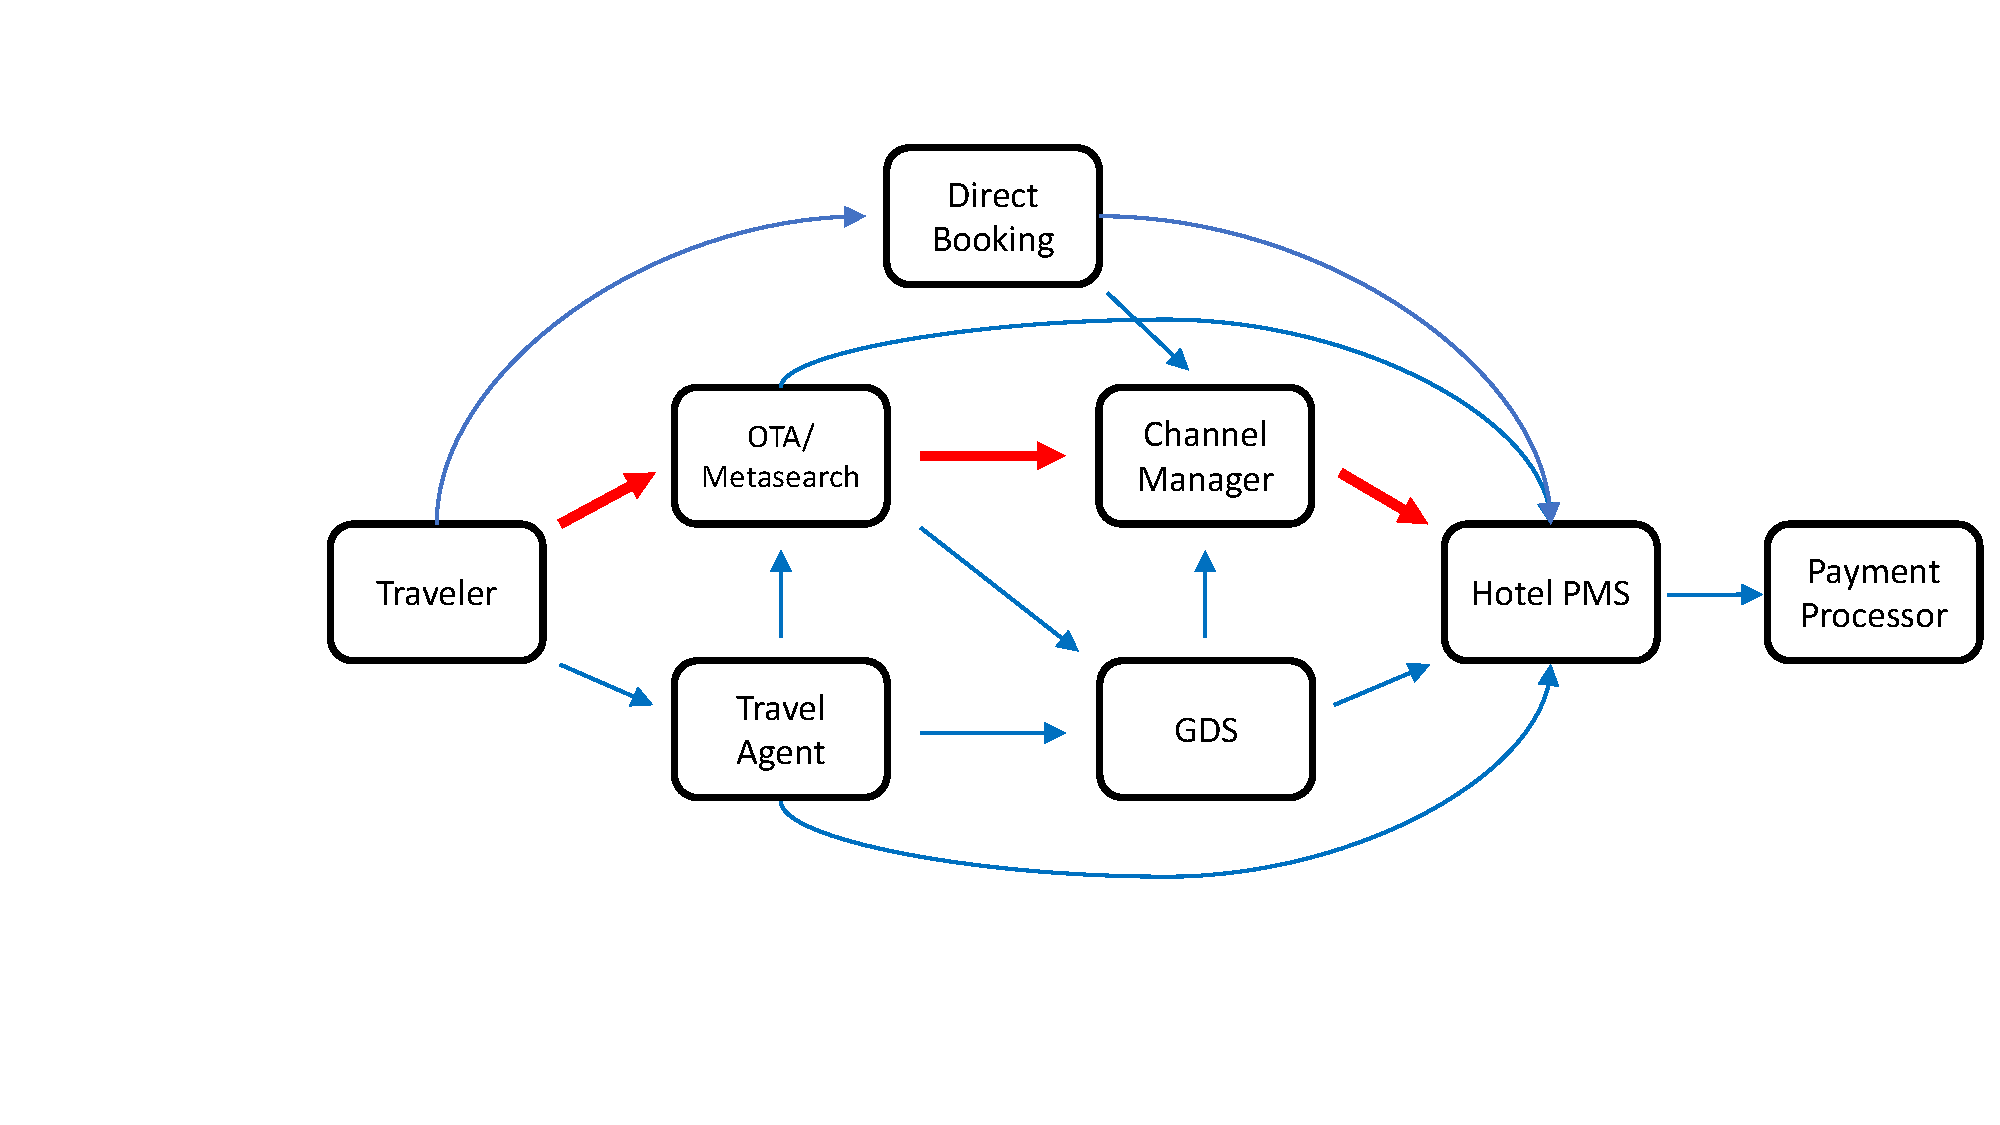
\includegraphics[width = \textwidth]{hotelEcosystem.pdf}
\caption{Current Ecosystem}
\label{fig1}
\end{figure}

\subsection{Players}
We describe the main players in the ecosystem by including a brief history and discussing the value they add and cost they subtract from the industry. 

\subsubsection{Travel Agent}
Travel agents appeared first as an intermediary between travelers and hotels in order to facilitate trip planning. While the internet has left brick and mortar travel agencies largely obsolete, they do still exist and are often helpful in booking group trips.
\begin{itemize}
 \item \underline{\textit{Value:}} Travel agents at their best will remove the burden of research and planning from the customer and provide individualized travel suggestions. Further, the hotel industry stands to benefit since the commission rates can be negotiated on a case by case basis.   
 \item \underline{\textit{Cost:}} Conflicts of interest may arise when the travel agent is secretly incentivized by higher paying hotels. In these cases, the traveler may not receive the best available deal for their preferences.
\end{itemize}

\subsubsection{Global Distribution System (GDS)}
Global distribution systems originally began in the airline industry (eAAsy Sabre) to provide a central platform for airlines and travel agents to aggregate flight data. By 1991, the Hotel Reservation Network (now Hotels.com) was founded to extend this idea directly to the customer for hotel bookings using a toll-free phone number. Currently, global distribution systems are largely outdated and seeking ways to reinvent themselves since online travel agents are now able to bypass their networks and work directly with the service providers (i.e hotels, airlines, and rental car companies).
\begin{itemize}
 \item \underline{\textit{Value:}} The benefit of a global distribution system lies in it's network and the consequent ability to bundle airline deals with hotel and car rental service providers. However, online travel agents (OTAs) are now able to provide the same service directly to the traveler which has left global distribution systems looking for ways to stay relevant.
 \item \underline{\textit{Cost:}} Availability and pricing information can be slow and spotty since global distribution systems typically act between service providers and travel agents rather than communicating directly with the travelers. 
\end{itemize}

\subsubsection{Online Travel Agent (OTA)}
Online travel agents represent the most dramatic change to the travel industry in the last decade. Initially, OTAs tapped directly into the GDS networks to find availabilities and sell directly to the interested traveler, however, channel management software packages now allow OTAs the option of bypassing the GDS and learning of availability information directly from the hotel or other service provider. While much of this has truly improved the travelers experience only two main parent companies currently exist - Priceline Group and Expedia Inc. - each with many subsidiary companies that creates the illusion of competion. This duopoly has predictably led to high commission rates and uneven legal agreements, the burden of which is shared by the hotel and the traveler in the form of lower profit and higher rates.
\begin{itemize}
 \item \underline{\textit{Value:}} Online travel agencies are easy to use and can provide discounts when bundling a flight, room, and rental car. 
 \item \underline{\textit{Cost:}} High commission rates charged by OTAs and various payment reconciliation methods add costs to the hotel which ultimately falls, at least in part, to the traveler. Further, booking through an OTA complicates the resolution of any disputes between the hotel and traveler (i.e. if a traveler is unsatisfied with the room and wants a discount they often must go through the OTA rather than working directly with hotel management). And finally, the sheer size of the two main OTAs allow for uneven and inconsistent legal agreements. 
\end{itemize}

\subsubsection{Channel Manager}
Channel management software allows the hotel to automatically update their availability and pricing information across their distribution network. This technology relies on two-way XML communication to push and pull data between the hotel's property management system and various booking platforms (i.e. online travel agents, global distribution system, direct booking through hotel's website) to help prevent over booking. It was the advent of this ability that ultimately allowed online travel agencies to bypass the global distribution system's information network and take hold of the market. 
\begin{itemize}
 \item \underline{\textit{Value:}} Automates much of the hotel's inventory planning and centralizes access to various distribution channels. 
  \item \underline{\textit{Cost:}} Most channel management companies operate on the software as a service (SaaS) model which further increases the hotel's operating cost and adds complexity into the hotel ecosystem. 
  \end{itemize}

\subsubsection{Property Management System (PMS)}
The hotel's property management system (PMS) refers to any piece of software designed to help manage the daily requirements of running a hotel. At it's most basic, a PMS will include functions to manage guest arrivals and departures and then generate the necessary reports for auditing. More advanced systems can include a housekeeping module, payment processor, and revenue management tools. 
\begin{itemize}
 \item \underline{\textit{Value:}} A good property management system can make the life of a hotelier much easier by automating and centralizing many of the daily operations. 
  \item \underline{\textit{Cost:}} Lack of customization and complicated interfaces makes it difficult to train new workers. 
  \end{itemize}

\newpage

\subsection{Proposed Ecosystem}
Since BookLocal will act as a property management system, channel manager, and payment processor for the hotel and provide metasearch capabilities for the traveler, much of the current ecosystem can be bypassed. As such, figure \ref{bl} represents our vision after full implementation. 

\begin{figure}[H]
\centering
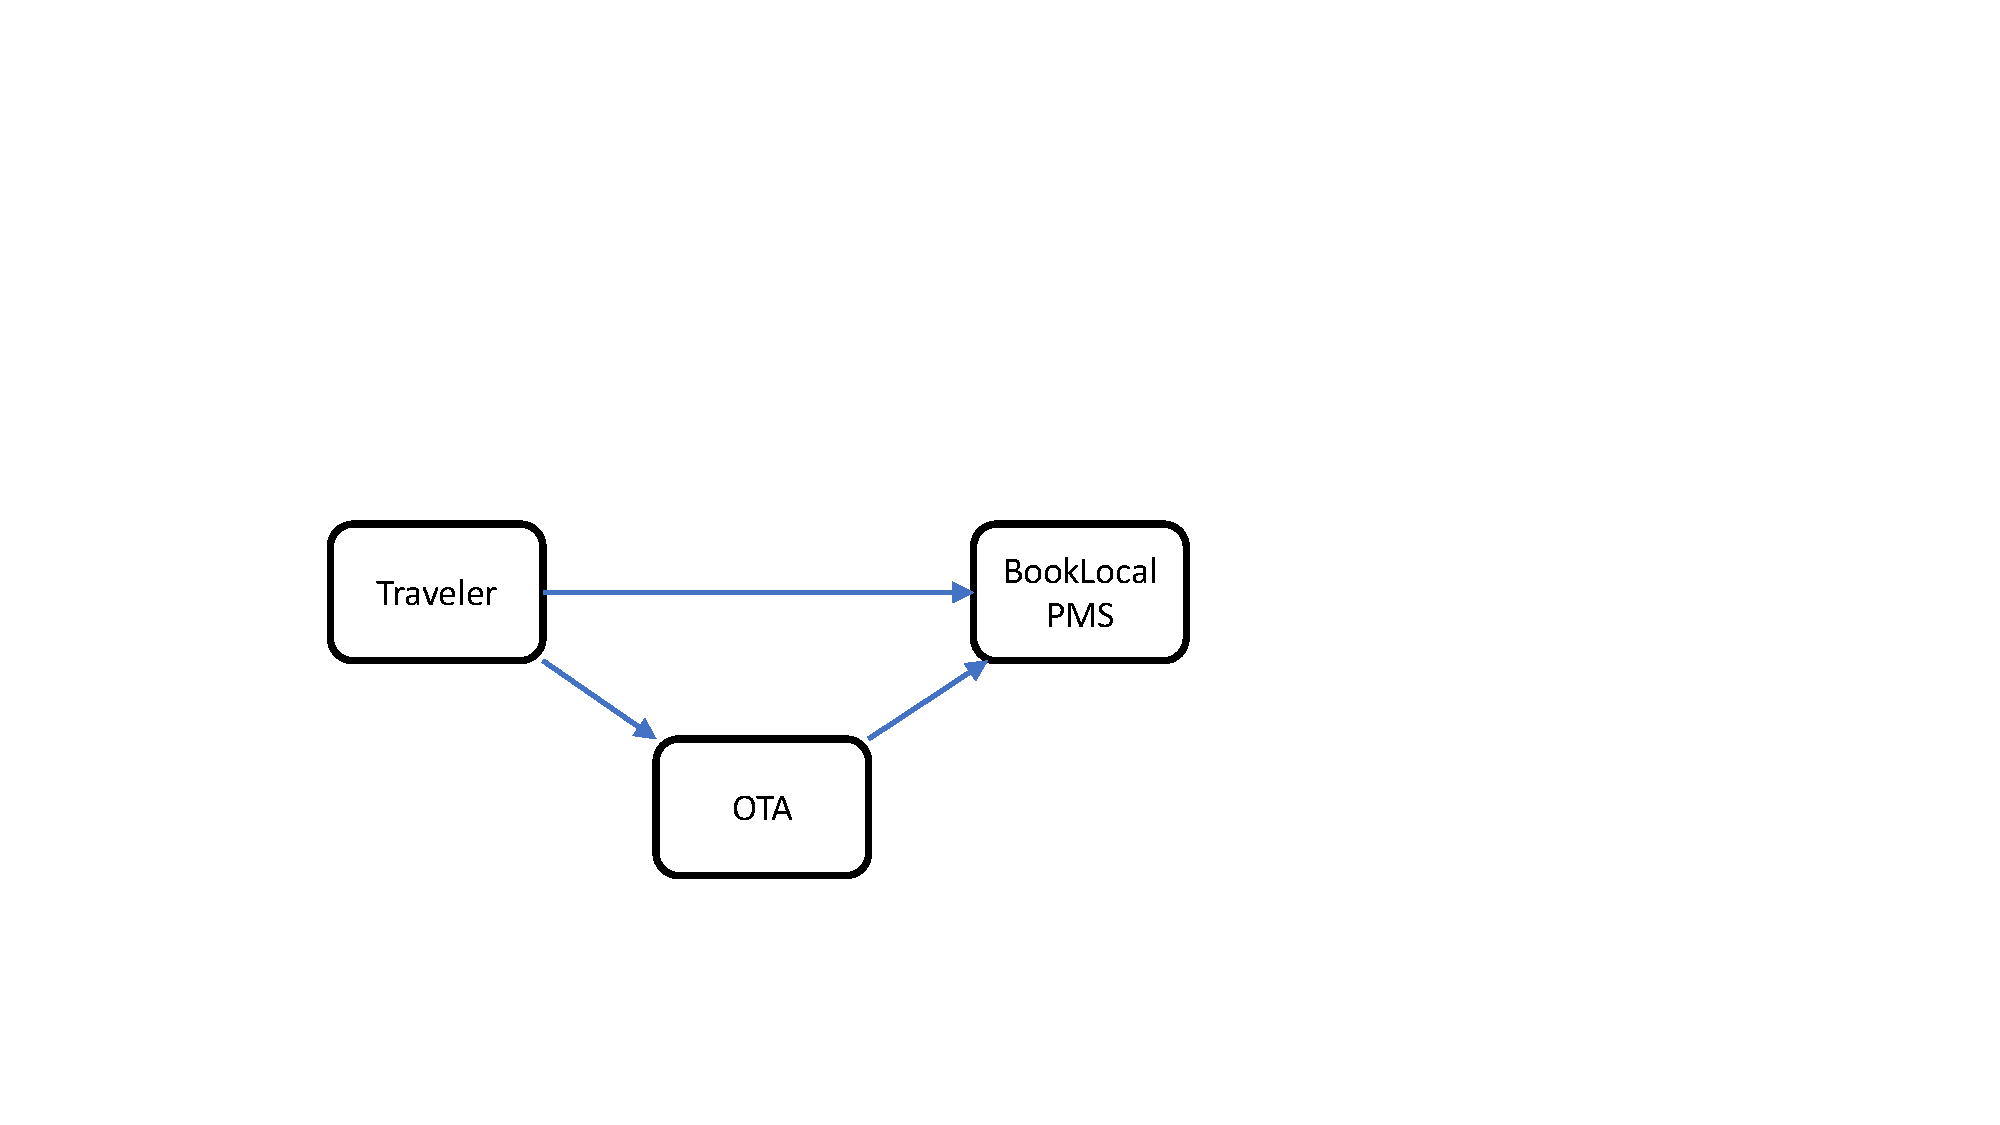
\includegraphics[width = .9\textwidth]{bookLocal_Ecosystem.pdf}
\caption{Proposed ecosystem}
\label{bl}
\end{figure}

\begin{flushleft}
Note that BookLocal seeks to be fully compatible with current online travel agencies in order to provide seamless integration for early-adopting hotels and late-adopting travelers.
\end{flushleft}

% ******************** HOW ********************
\newpage
\section{How}
The heart of BookLocal will reside in a series of smart contracts on the public Ethereum blockchain. 
\subsection{Data}
BookLocal will maintain it's own plasma subchain to handle the bulk of the transactional data. This will minimize the number of updates to the main Ethereum chain and thus save in transaction fees. Further, upon making a reservation, a new subchain will be created for the hotel guest (a traveler who commits to a hotel becomes a guest) and will terminate upon checkout whereby the final balances are settled. Visually we represent the flow of data below:

\begin{figure}[H]
\centering
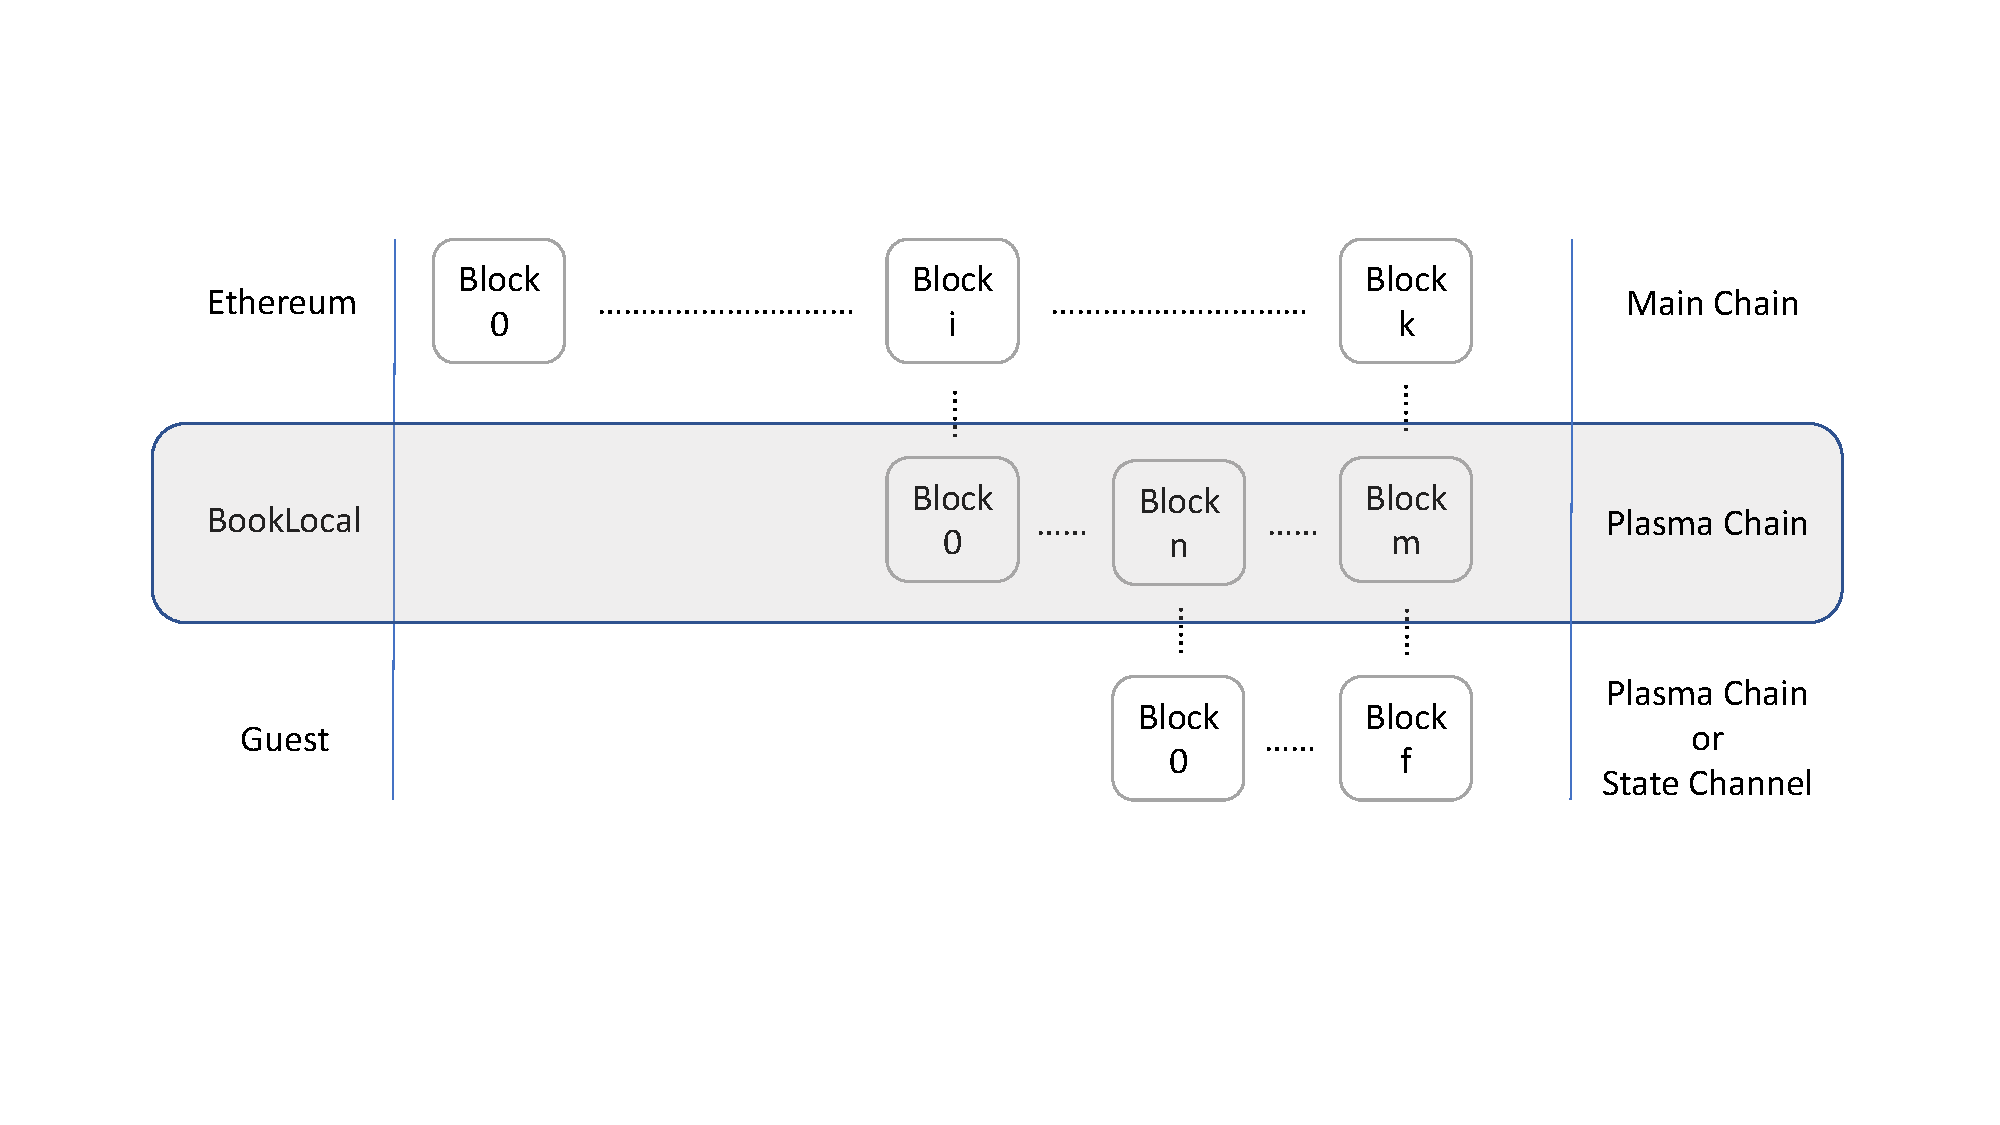
\includegraphics[width = \textwidth]{bookLocal_dataLayers.pdf}
\end{figure}

\subsection{Traveler}
With BookLocal, the traveler will be able to search, compare, and book a hotel room. Additionally, we will incorporate a wallet feature that allows the guest to use their phone to pay for dinner, events, or other travel related activities.  

\subsubsection{Search}
The search feature will be a read only function (i.e. constant insofar as it cannot update the blockchain) that searches for available rooms during your travel. Our vision for this feature is to allow the guest to search the hotel in a visually intuitive manor whereby they can view the hotel, select the floor, and finally look at a view of the entire floor plan to select from available rooms. This feature gives control to the traveler to decide exactly which room and view they want. 

\subsubsection{Compare}
Compare will again be a read only function that allows the traveler to select some number of rooms or hotels to compare side by side. This can include reviews and pictures from other guests as well as more formal descriptions from the hotel itself.

\subsubsection{Book}
When the traveler has found a room they like, they can book the room in one of several ways: 
\begin{itemize}
 \item Send exactly the asking rate.
 \item Send more than the asking rate and use the BookLocal wallet to pay for food and activities during the trip. This works as a budgeting commitment device to ensure you don't overspend during your trip. 
 \item Send some amount less than the upfront asking rate (if booking well in advance) to hold your room for a period of time and pay the remainder closer to the actual check-in date. This option will likely cost more due to the convenience. 
\end{itemize}
No matter which option the traveler chooses, each new reservation will create a plasma side chain (or state channel) that can only be edited by the hotel and the guest. Upon checkout the final balances are recorded and the chain will be terminated. Use of a plasma chain for each guest would afford the option of selling their detailed trip data to interested parties. 

\begin{flushleft}
Since the act of booking a room will change the availability and options for other travelers, each transaction with this function will require updating data on the BookLocal plasma chain. 
\end{flushleft}

\subsubsection{Purchase}
The purchase function will act as a simple wallet enabling the guest to pay for food, drinks, and events in the local ecosystem. 

\begin{flushleft}
To give an example: let's say a traveler, Ann, is willing to spend at most \$400 for a day and night in Paris. She uses BookLocal to find a hotel that costs \$100 per night and decide to book. Since she already knows her desired budget for the weekend, she chooses to book the room by transferring all \$400 to the BookLocal holding address. A new subchain is created for her stay which now includes \$300 in the wallet to spend in Paris (\$400 less \$100 for room). Now Ann is able to use the BookLocal app to eat, shop, go to museums, and so on. If at the end of her trip she only spent \$250 in total (including room), and there are no room disputes or damages, then the remaining \$150 that she didn't spend will be immediately returned to her upon checkout.
\end{flushleft}

\subsection{Hotel}
The hotel interface will require the following functionality:  

\subsubsection{Guest Management}
Guest management includes managing arrivals and departures with any special requests. Sub features involve messaging capability between the guest and hotel and a variety of viewing options to see arrivals and departures for different time scales (i.e. monthly view, weekly view, daily view, and so on).

\subsubsection{Housekeeping and Maintenance}
The housekeeping module will include messaging capabilities, room specific cleaning details, a scheduled order and cleaning assignments, and requests for supplies and maintenance repairs.

\subsubsection{Revenue Management}
Revenue management will act as a recommendation system to provide different pricing options during peak hours or otherwise. 

\subsubsection{Payment Processor}
Upon checkout, BookLocal will finalize the guest's plasma chain (or state channel), record the final balances, and transfer funds accordingly. This module will need to work seamlessly for someone paying with a credit card and incorporate a point of sale system with inventory management for hotel purchases (i.e. drinks, snacks, toiletry items, and so on).

\subsubsection{Report Generator}
This module will generate industry specific reports used during night audits as well as provide real time key performance indicators.  

\subsubsection{Channel Management}
In order to feasibly integrate into the current ecosystem, BookLocal will include channel management functionality to allow travelers the option of booking through an online travel agency while still creating a guest specific subchain on BookLocal.   

\subsection{Dispute}
In case of a disputed room charge or rate, the guest or hotel can open a dispute. Both the guest and hotel will have a specified amount of time (i.e. two-weeks) to submit their claim after which BookLocal will make the final decision. Here, the guest's subchain stays open and unresolved until BookLocal's decision.


% ******************** STEPS ********************
\newpage
\section{Steps}
Below are the key benchmarks toward full adoption. 
\subsection{Exchange Hotel}
The Exchange Building in Memphis, Tennessee will host the first version of BookLocal as it's own proprietary property management system. 
\subsection{Independent Hotels}
Once the BookLocal platform is successfully tested at the Exchange Building, we will open up the application for use at other independent hotels.
\subsection{Chain Hotels}
Finally, we will target chain hotels by adding permissioned network features to allow for corporate oversight on overall and hotel specific performance.


\end{document}


% Figures
\begin{figure}[H]
\centering
\includegraphics[width = .9\textwidth]{}
\caption{}
\end{figure}

% Paragraph
\begin{flushleft}
\end{flushleft}

